\documentclass{beamer}
\usepackage[utf8]{inputenc}
\usepackage[frenchb]{babel}
\usepackage{tikz}
\usetikzlibrary{shapes,positioning,snakes,calc}
\usetheme{Warsaw}

\def\android{Android\texttrademark}

\title{FMIN200 \\ TER~: Reconception du jeu PtiClic sous \android{}}
\author{DUPÉRON Georges \and\\ CHARRON John \and\\ BRUN Bertrand \and\\ BONAVERO Yoann}
\institute{Université Montpellier II, Département informatique}
\date{Lundi, 23 mai 2011}

\begin{document}

\begin{frame}
  \titlepage
\end{frame}

\section{Le Jeu}
\begin{frame}
 \begin{minipage}{\textwidth}
   \centering 
   partie droite
 \end{minipage}
 \begin{minipage}{\textwidth}
   \centering 
   partie gauche
 \end{minipage}
\end{frame}

\begin{frame}
% bertrand
 Caractéristique d'\android{}~:
  \begin{itemize}
    \item<+-> fondé sur un noyau Linux
    \item<+-> interface de programmation en Java (Dalvic VM)
    \item<+-> basé sur le modéle MVC
  \end{itemize}
\end{frame}

\begin{frame}
  Le framework~:
  \begin{itemize}
    \item<+-> SDK
    \item<+-> Emulateur
    \item<+-> Plugin Eclipse
  \end{itemize}
\end{frame}

\begin{frame}
  Le developpement~:
  \begin{itemize}
    \item<+-> Le patron de conception MVC (Modele-Vue-Controlleur) % mettre schema MVC Propre a Android
  \end{itemize}
\end{frame}

\begin{frame}
  Planning
  \begin{itemize}
  \item planning initial~: quatre itérations
  \item planning réel~: deux itérations
  \end{itemize}
\end{frame}

\begin{frame}
  Planning : deux itérations = 2 prototypes
  \begin{itemize}
  \item prototype Android Java
  \item prototype Smartphone
  \end{itemize}
\end{frame}

\begin{frame}
  % Georges
  \begin{tikzpicture}[
    mynode/.style = {circle, minimum size=1.5cm},
    mc/.style = {mynode,draw=red,text=red},
    mn/.style = {mynode,draw},
    mi/.style = {mynode,draw=gray,text=gray},
    rel/.style = {font=\footnotesize},
    guess/.style = {->,dashed},
    exist/.style = {->},
    auto,swap
    ]
    \node[mc] (mc) {Chat};
    \node[mn] (mn0) at (0,3) {Souris};
    \node[mi] (mi1) at (3,-2) {matou};
    \node[mn] (mn2) at (6,0) {animal};
    \path[exist] (mc) edge[bend right] node[rel]{idée associée} (mn0);
    \path[exist] (mc) edge node[rel]{synonyme} (mi1);
    \path[exist] (mi1) edge node[rel]{sorte de} (mn2);
    \path[guess,swap] (mc) edge node[rel]{sorte de ?} (mn2);
    \path[guess,swap] (mc) edge[bend left] node[rel]{\shortstack{sorte de ?\\synonyme ?\\\dots}} (mn0);
  \end{tikzpicture}
\end{frame}

\begin{frame}
  Ferdinand de Saussure (1857-1913), Cours de linguistique général
  \begin{itemize}
  \item Signe linguistique
  \item Arbitraire du signe
  \item Synchronie et diachronie
  \item Langue et Parole
  \end{itemize}
\end{frame}


\begin{frame}  
\begin{figure}[h!]
  \centering
      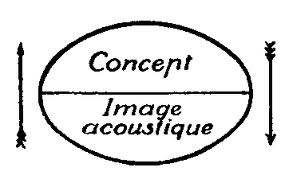
\includegraphics[width=0.5\textwidth]{img/signe-conceptimageacoustique.jpeg}
\end{figure}
\end{frame}

\begin{frame}
\begin{figure}[h!]
  \centering
      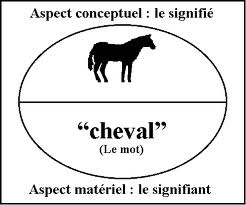
\includegraphics[width=0.5\textwidth]{img/signe-cheval.jpeg}
\end{figure}
\end{frame}

\begin{frame}
\begin{figure}[h!]
  \centering
      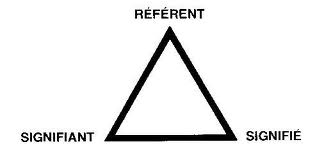
\includegraphics[width=0.5\textwidth]{img/trianglesemiotique.jpeg}
\end{figure}
\end{frame}

\begin{frame}
  Réseau lexical JeuxDeMots
  \begin{itemize}
  \item noeuds
  \item relations
  \end{itemize}
\end{frame}

\begin{frame}
  Réseau lexical JeuxDeMots~: types de noeuds
  \begin{itemize}
  \item termes
  \item catégories grammaticales
  \item informations métalinguistiques supplémentaires (types 18 et 36)
  \end{itemize}
\end{frame}

\begin{frame}
  Réseau lexical JeuxDeMots~: types de relations
  \begin{itemize}
  \item morphologique
  \item syntaxique
  \item sémantique
  \item pragmatique
  \item métalinguistique
  \end{itemize}
\end{frame}

\begin{frame}
  Réseau lexical JeuxDeMots~: quelques statistiques
  \begin{itemize}
  \item environ 45\% des noeuds ne sont pas liés à des relations sémantiques sortantes
  \item environ 70\% des noeuds ne sont pas liés à des relations sémantiques entrantes
  \end{itemize}
\end{frame}

\begin{frame}
  Réseau lexical JeuxDeMots~: bruits et silences
  \begin{itemize}
  \item bruits = relations plus fortes que la réalité 
  \item silence = relations non existantes ou trop faible par rapport à la réalité 
  \item bruits + silences = couverture de relations sémantiques hétérogènes
  \end{itemize}
\end{frame}


\begin{frame}
\begin{figure}
 \begin{minipage}{\textwidth}
\centering 
       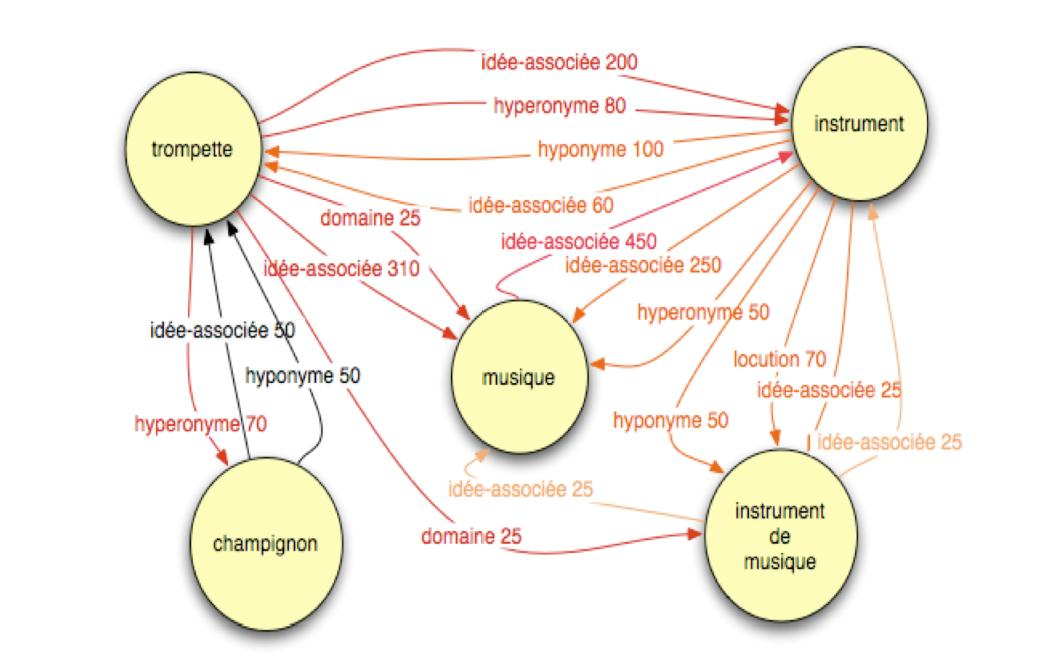
\includegraphics[width=0.75\textwidth]{img/jdm.jpeg}
    \end{minipage}
\end{figure}
\end{frame}


\begin{frame}
\begin{figure}
 \begin{minipage}{\textwidth}
\centering 
       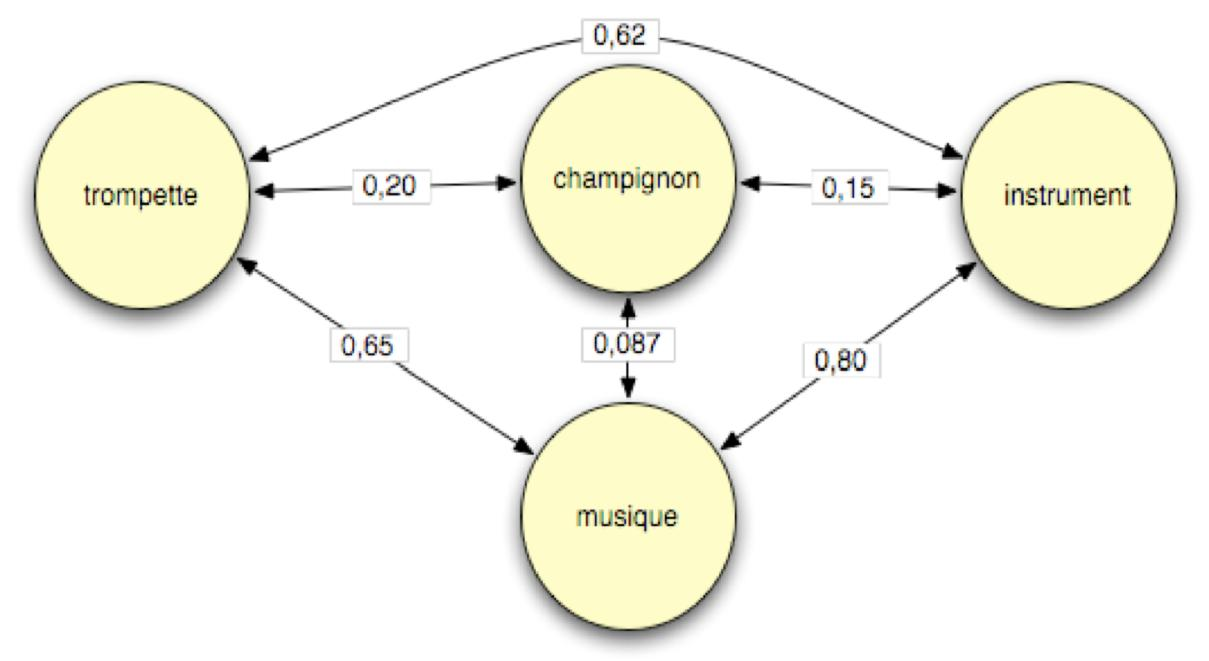
\includegraphics[width=0.75\textwidth]{img/lsa.jpeg}
  \end{minipage}
\end{figure}
\end{frame}


\begin{frame}
\begin{center}
        \begin{tabular}{ | l | l | l | l | p{5cm} |}
        \hline
RELATION &	'mc' & 'mn'	& 'remarques' \\ \hline
-1 => "'mn' n'est pas lié à 'mc'" &	adj, adv, noms, verbes & adj, adv, noms, verbes	& \\ \hline
0 =>  "'mc' est en rapport avec 'mn'" & adj, adv, noms, verbes & adj, adv, noms, verbes & \\ \hline
5 => "'mc' est un synonyme de 'mn'" & adj, adv, noms, verbes & adj, adv, noms, verbes & même POS \\ \hline
6 => "'mc' est une sorte de 'mn'" & noms & noms & \\ \hline
7 => "Un contraire de 'mc' est 'mn'" & adj, adv, noms, verbes &	adj, adv, noms, verbes & même POS \\ \hline
8 => "Un spécifique de 'mc' est 'mn'" & noms & noms & \\ \hline
9 => "'mn' est une partie de 'mc'" & noms & noms & \\ \hline
10 => "'mc' fait partie de 'mn'" & noms & noms & \\ \hline
13 => "Quoi/Qui pourrait 'mc'" & verbes & noms & \\ \hline
15 => "Le lieu pour 'mc' est 'mn'" & noms, verbes & noms (lieu NON!!) & \\ \hline
16 => "Un instrument pour 'mc' est 'mn'" & verbes & noms & \\ \hline
17 => "Un caractéristique de 'mc' est 'mn'" & noms & adj & \\ \hline
        \end{tabular}
\end{center}
\end{frame}

\begin{frame}
  \begin{itemize}
  \item Site web
    \begin{itemize}
    \item Présentation de l'application
    \item Le jeu
    \end{itemize}
  \item Page de création de parties
    \begin{itemize}
    \item Architecture
    \item Bonus
    \end{itemize}
  \end{itemize}
\end{frame}

\begin{frame}
  % Georges
  \texttt{\textcolor{gray}{http://pticlic.fr/jeu.html}\#\textcolor{red}{game}/\textcolor{blue}{1306104746953}/\textcolor{blue}{5,0,5,-1}}
  \vskip 1em%
  \begin{tikzpicture}[
    state/.style = {circle,draw,minimum size=1.5cm},
    transition/.style = {->},
    event/.style = {->, decorate, decoration={snake, post length=.5mm}, segment amplitude=.4mm, segment length=2mm},
    source/.style = {},
    auto,
    secondary/.style={draw=gray}
    ]
    \node[state] (goto) {goto};
    \node[left=of goto] (arbitrary) {$*$};
    \node[state, right=of goto] (pre-enter) {\shortstack{pre-\\enter}};
    \node[state, right=of pre-enter] (enter) {enter};
    \node[state, right=of enter] (update) {update};
    \node[state, below=of goto] (leave) {leave};
    \node[coordinate, below=of pre-enter] (c1) {};
    \node[coordinate, below=of enter] (c2) {};
    \node[state] (ajax) at ($0.5*(c1) + 0.5*(c2)$) {AJAX};
    \node[source, above=of goto] (hash) {hashchange};

    \draw[transition] (goto) edge node {2} (pre-enter);
    \draw[transition,dashed] (pre-enter) -- (enter);
    \draw[transition] (enter) -- (update);
    \draw[transition] (goto) edge node {1} (leave);
    \draw[event,draw=red] (hash) -- (goto);
    \draw[event] (arbitrary) -- (goto);
    \draw[event] (arbitrary) to[out=90, in=225] (hash.south west);
    \draw[event,secondary] (pre-enter) -- (ajax);
    \draw[event,secondary] (ajax) -- (enter);
    \draw[event,draw=blue] (hash.east) to[out=0, in=135] (update);
  \end{tikzpicture}
\end{frame}

\begin{frame}
Conclusion
\begin{itemize}
  \item reste à faire
  \item alpha tests
  \item situation réelle de réalisation de projet
  \end{itemize}
\end{frame}

\begin{frame}
\centering
Merci de votre attention... \\
Avez-vous des questions~?
\end{frame}

\end{document}

